\chapter{Cloud storage}
After going through CPU and network virtualization, it's time to talk about
proper ways of handling storaged data. In the age of \emph{cloud computing}
there's a huge amount of data to store, access and secure, so novel approches
to system design are necessary. To achieve the goal of cloud computation,
effective data replication and appropriate storage management strategies are
critical.

In the past, storage systems were designed according to a
\emph{performance-at-any-cost} philosophy, but now there's been a shift towards
\emph{reliability-at-the-lowest-possible-cost}. For example, data replication
allows concurrent access to data from multiple processors and decreases the
chances of data loss, but maintaining consistency among multiple copies of data
records increases complexity of the management software, and could negatively
affect the storage system performance as a whole, if data is frequently updated.

In this chapter we're going to explain some modern strategies adopted
to manage cloud storage while also respecting performance and realibility
requirements.

\section{Preliminary definitions}
Before proceding, we need to fix some concepts.

\begin{definition}[Storage model]
    A storage model describes the layout of a data structure in a physical storage.
\end{definition}
\begin{definition}[Data model]
    A data model captures the most important logical aspects of a data structure
    in a database 
\end{definition}

\begin{definition}[Read-write coherence]
    The result of reading by a memory cell, should be the same as the most recent
    writing done on that cell.
\end{definition}
\begin{definition}[Before-or-after atomicity]
    The result of every read or write operation is the same as if that
    operation has been performed completely before or after another read or
    write operation.
\end{definition}

\noindent
\emph{Read-write coherence} and \emph{Before-or-after atomicity} are two highly
desirable properties of any \emph{storage model}.

\subsection{Types of storage}
There are three main types of storage:
\begin{enumerate}
    \item \emph{Block storage}: data is managed as blocks within sectors and
    tracks. Can be used when storage has access to raw and unformatted hardware
    and is useful when both speed and efficiency are important;
    \item \emph{File storage}: data is organized as structured files which are
    managed through a file system. However, this doesn't work very well with
    large amounts of data or when there's high-demand for a particular piece
    of data;
    \item \emph{Object storage}: data is managed as objects. Typically, each
    object has a global unique identifier and holds both the data itself and
    some metadata. It's possible to access whole objects or blobs of data, but
    random accesses to data within an object is more difficult;
\end{enumerate}

\noindent
\emph{Block storage} is often used for database because it's the ideal way of
storing relational information. On the other hand, \emph{Object storage} isn't
suitable for databases, but is preferable to store content that can grow without
bounds, for example, backups and archives. Finally, the \emph{File storage} model
can be easily used to create \emph{distributed file systems} via network protocols.

Examples of \emph{Block storage}, \emph{File storage} and \emph{Object storage}
are, respectivelly, \emph{Cinder}, \emph{Google file system} and \emph{OpenStack
Swift}.

\section{Block storage}
We'll give a first quick look to this model by scratching the surface of
\emph{OpenStack Cinder}. \emph{OpenStack Cinder} implements services and libraries
to provide on-demand, self-service access to block storage resources. It provides
API to interact with storage backends which is also exposed to the cloud. End
users can manage their storage without knowing how it's organized and for both
physical and virtual environments.

\begin{figure}[h!]
    \centering
    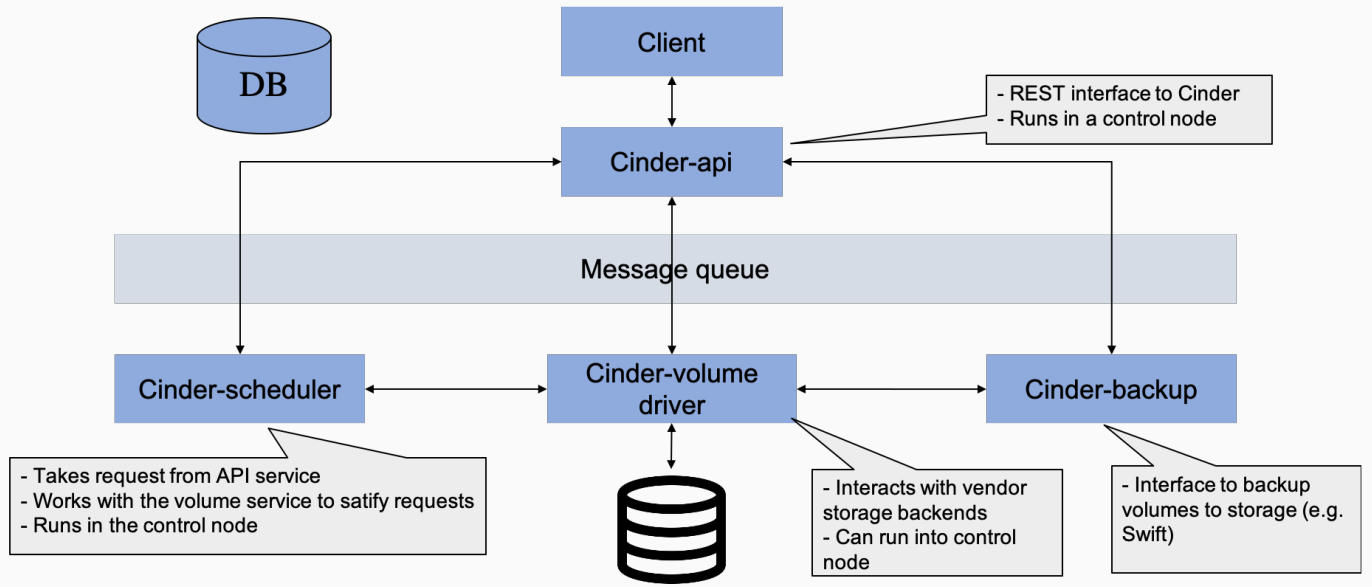
\includegraphics[width=0.7\textwidth]{images/block-model-cinder.png}
    \caption{\emph{OpenStack Cinder} basic architecture}
\end{figure}

\noindent
\emph{Cinder} APIs allow users to create and delete volumes and snaphots (for
backup pourposes). Attach or detach volumes for the available storage, clone and
extend them, and so on.

\section{Distributed file system}
Again, we'll start by giving some definitions.

\begin{definition}[File]
    A file is a linear array of cells stored on a persistent storage device. It
    is seen by application as a collection of logical records, and it's stored
    on a physical device as a set of physical records, or blocks, whose size
    is dictated by the physical media.
\end{definition}
\begin{definition}[File pointer]
    A file pointer is a cell used as starting point for a read or write operation.
\end{definition}

\noindent
A file has a logical organisation that reflects the \emph{data model} from the
perspective of the application, and a physical orgnisation that reflects the
\emph{storage model} and describes the manner the file is stored on a given
storage media.

\begin{definition}[File system]
    A file system is a collection of directories and each directory provides
    information about a set of files. A file system controls how data is stored
    and retrieved.
\end{definition}

\subsection{Unix File System}
The \emph{Unix File System} (\emph{UFS}) has both a layered and hierarchical
design. The first allows it to separate the physical file structure from the
logical one, and this becomes useful when dealing with files stored both locally
and remotely. The hierarchical design, on the other hand, allows grouping of
files in directories, and supports multiple levels of directories, or collections
of directories and files; thus, supporting a good degree of scalability.

The metadata that \emph{UFS} uses includes file owner, access rights, creation
time, time of the last modification, file size, the structure of the file and
the persistent storage device cells where data is stored. All of these are
memorized in a structure called \emph{inode}. Each \emph{inode} holds information
about individual files and directories and is kept on persistent media together
with the actual data.

\bigskip\noindent
Going back to \emph{UFS} layering, there are two layers:
\begin{itemize}
    \item \emph{Lower layer}: is about the physical organisation and is furderly
    separated into three sub-layers:
    \begin{itemize}
        \item \emph{Block layer}: responsible for locating individual blocks on
        the physical device;
        \item \emph{File layer}: reflects the organisation of blocks into files;
        \item \emph{Inode layer}: provides metadata for files and directories;
    \end{itemize}
    \item \emph{Upper layer}: is about the logical orgnisation;
\end{itemize}

\newpage
\begin{figure}[ht!]
    \centering
    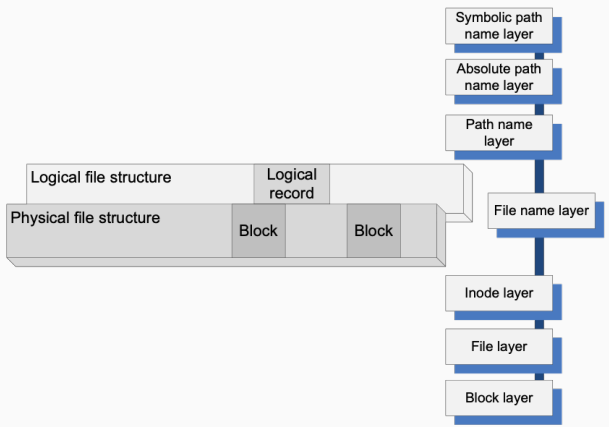
\includegraphics[width=0.6\textwidth]{images/ufs-layering.png}
    \caption{\emph{UFS} layering}
\end{figure}

\subsection{Network File System}
The \emph{Network File System} (\emph{NFS}) is designed to provide the same
semantics as the \emph{UFS} to ensure compatiblity with existing applications.
\emph{NFS} is based on the client-server paradigm. Clients run on the local host
and interact with the server via remote procedure calls.

Each remote file is identified by a 32-bit file handler rather than a file
descriptor like in \emph{UFS}. A file handler is obtained combining a file
system identication, an \emph{inode} number and a generation number.

\begin{figure}[h!]
    \centering
    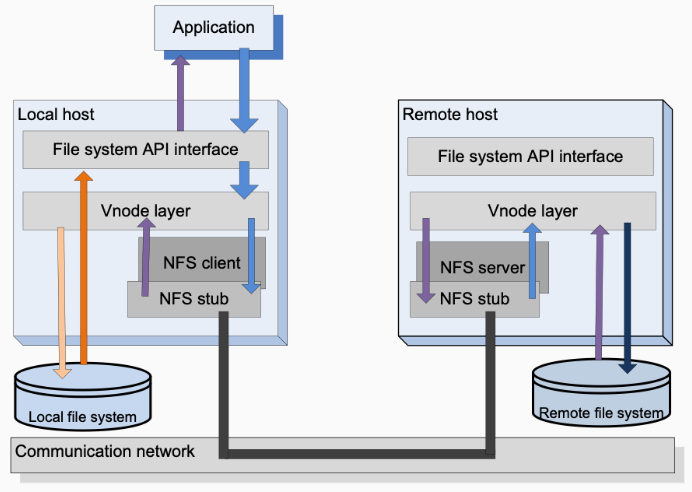
\includegraphics[width=0.6\textwidth]{images/nfs-design.png}
    \caption{\emph{NFS} design}
\end{figure}

\noindent
As the image shows, instead of an \emph{inode layer} the \emph{NFS} has a
\emph{vnode layer} which implements file operations in a uniform manner,
regardless of whether the file is local or remote. Also, an operation targeting
a local file is directed to the local file system without involving the \emph{NFS}.

When a client interacts with the server, the client-side \emph{NFS} packages the
relevant information about the target, then sends those packaged information to
the server-side \emph{NFS}. The latter then passes the received information to the
\emph{vnode layer} of the remote host which finally directs it to the remote
file system.

\newpage
\begin{table}[ht!]
    \centering
    \begin{tabular}{|l|l|c|l|p{0.5\textwidth}|}
        \hline
        \textbf{API} & \textbf{Description} && \textbf{API} & \textbf{Description}\\
        \hline
        \texttt{fd} & File descriptor && \texttt{dfh} & The directory in which the file
        handle can be found\\
        \hline
        \texttt{fh} & File handle && \texttt{count} & Number of bytes to be transferred\\
        \hline
        \texttt{fname} & File name && \texttt{buf} & Buffer used to transfer data\\
        \hline
        \texttt{dname} & Directory name && \texttt{device} & The device in which the
        file system is located\\
        \hline
    \end{tabular}
    \caption{\emph{NFS} APIs}
\end{table}

\begin{figure}[h!]
    \centering
    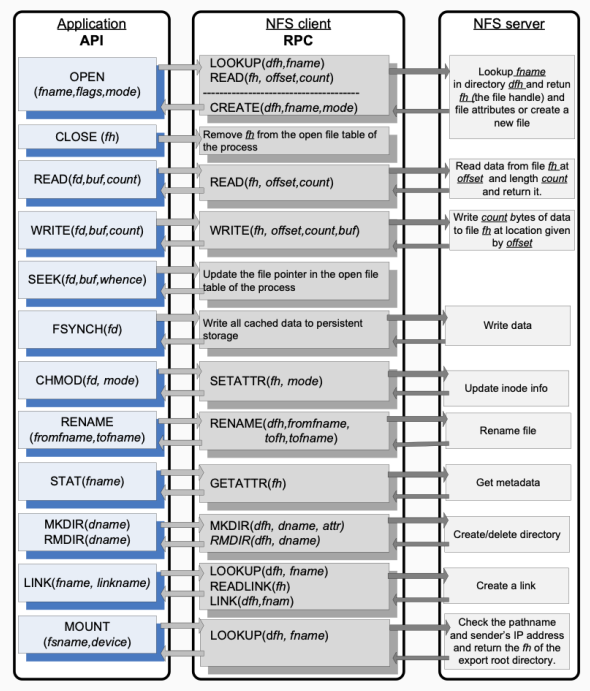
\includegraphics[width=0.6\textwidth]{images/nfs-remote-calls.png}
    \caption{\emph{UFS} APIs and corresponding \emph{NFS} remote procedure calls}
\end{figure}

\paragraph{Common design choices for distributed file system}
The vast majority of distributed file systems have been implemented in similar
a way. That's not so surprising if we think that they all need to solve the same
problems and that the possibles or best solutions to choose from are limited.

Tipically, every distributed file system is implemented in a way that once a file
is closed, the server will have the newest version of it on persisten storage.
Another concern is about what to do when writing on a file. The possible
approches are two:
\begin{enumerate}
    \item \emph{Write-through}: a block is written to the disk as soon as it is
    available on the cache. This approch increases reliability, but it takes more
    time to complete each write operation;
    \item \emph{Delay in write-back}: a block is first written to cache and
    writing on the disk is delayed for a time in the order of tens of seconds.
    This speeds up writings and avoids useless writings when data is discarded
    before saving on disk is necessary. However, data can be lost in case
    of system failures;
\end{enumerate}

\noindent
Finally, how should the system act when multiple clients tries to access the
same file at the same time? The possibilities are two:
\begin{enumerate}
    \item \emph{Sequential write-sharing}: a file cannot be opened simultaneously
    for reading and writing by several clients;
    \item \emph{Concurrent write-sharing}: multiple clients can modify the same
    file at the same time (in a concurrent way, of course);
\end{enumerate}

\subsection{General Parallel File System}
\emph{General Parallel File System} (\emph{GPFS}) is a distributed file
system developed by IBM that's designed for optimal performance of large
clusters. To do so, it allows parallel I/O, meaning that multiple I/O
operations can be executed concurrently.

\begin{figure}[h!]
    \centering
    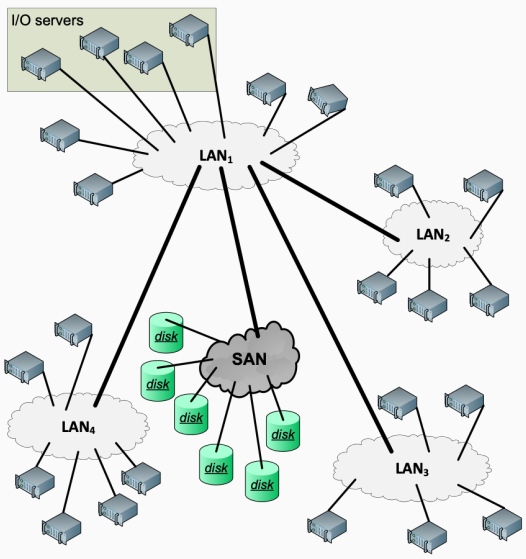
\includegraphics[width=0.6\textwidth]{images/gpfs-design.png}
    \caption{\emph{GPFS} architecture}
\end{figure}

\noindent
As the image shows, every disk is interconnected via a \emph{Storage Area Network}
(\emph{SAN}) and servers used to handle I/O are distributed in various LANs.

\emph{GPFS} is a realiable file system because it can recover from system
failures. To achive so, \emph{GPFS} records all metadata updates in a write-ahead
log file. Write-ahead means that updates are written to persistent storage only
after log records have been written. Every I/O node manages one log file for
each file system it mounts and any I/O node can initiate recovery on behalf of
a failed node.

Finally, \emph{GPFS} uses data striping to allow concurrent access and improve
performance. By using data striping, \emph{GPFS} segments logically sequential
data (e.g. files) so that consecutive segments are stored on different physical
storage devices. The problem with this approch is that a failed disk will affect
many more files. To reduce the impact of this and further improve fault tollerance,
\emph{GPFS} data files as well as metadata are replicated on two different
physical disks.

\subsection{Google File System}
\emph{Google File System} (\emph{GFS}) is another distributed file system,
developed by Google that uses thousands of storage devices built from inexpensive
commodity components to provide PBs of storage to a large user community
with various needs.

\begin{table}[h!]
    \centering
    \begin{tabular}{|p{0.47\textwidth}|p{0.47\textwidth}|}
        \hline
        \textbf{Design consideration} & \textbf{Design choice}\\
        \hline
        Vast majority of files range in size from a few GBs to hundreds of TBs &
        Files are segmented in large \emph{chunks}\\
        \hline
        Most common operation is to append to an existing file and random write
        operations to a file are extremely infrequent & Implement an atomic file
        append operation allowing multiple applications operating concurrently
        to append to the same file\\
        \hline
        Consistency model should be relaxed to simplify the system implementation
        but without placing an additional burden on application developers &
        Ensure consistency by channeling critical file operations through a
        \emph{master}, a component of the cluster which controls the entire
        system\\
        \hline
    \end{tabular}
\end{table}

\noindent
Other considerations made are:
\begin{itemize}
    \item Scalability and reliability are critical features of the system, and
    they must be considered from the beginning, rather than at some stage of the
    design;
    \item Sequential read operations are the norm;
    \item Users process the data in bulk and are less concerned with the
    response time;
\end{itemize}
And other relevant design decisions are:
\begin{itemize}
    \item Clusters must be built around a high-bandwidth rather than a low-latency
    interconnection network, so control and data flows should be separated.
    High-bandwidth data flow should be scheduled by pipelining data transfer over
    TCP connections and finally, the network topology should be exploited by
    sending data to the closest node in the network;
    \item Caching at client side should be eliminated to reduce the overhead
    that's necessary for maintaining consistency among cached copies;
    \item Efficient checkpointing and fast recovery mechanisms should be
    supported as well as an efficient garbace colletor;
\end{itemize}

\paragraph{GFS chunks}
So, as we said, files are segmented into large \emph{chunks}. To be more precise,
each \emph{chunk} is large exactly 64MB. This choice was motivated by the desire
to optimize performance for large files and to reduce the amount of metadata
maintained by the system. Also, large \emph{chunk} size increases the likelihood
that multiple operations will be directed to the same \emph{chunk}; thus it
reduces the number of requests to locate the \emph{chunk} and also allows
applications to maintain a persistent network connection with the server where
the \emph{chunk} is located.

A \emph{chunk} is then divided in 64KB blocks and each block holds a 32bit
checksum. Each \emph{chunk} is stored in a \emph{UFS} and is replicated on a
configurable amount of sites (default is 3 replicas). At the time of creation,
each \emph{chunk} is given a unique \emph{chunk} handle.

\paragraph{GFS architecture}
The following image shows the typical architecture of a \emph{GFS} implementation.
Each \emph{master} maintains state information about all system components and
control a number of \emph{chunk servers}. A \emph{chunk server} is basically a
Linux system and uses metadata provided by its \emph{master} to communicate
directly with the applications.

\begin{figure}[ht!]
    \centering
    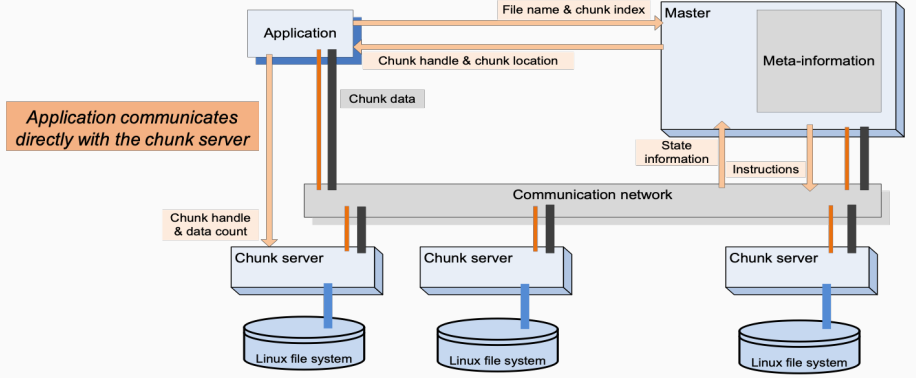
\includegraphics[width=0.6\textwidth]{images/gfs-architecture.png}
    \caption{\emph{GFS} architecture}
\end{figure}

\begin{note}
    Data and control flows have been graphically separated.
\end{note}

\paragraph{Steps for a write request}
Let's see the steps required to complete a generic write operation.
First, the client contacts the \emph{master} which replies with the location
of the primary and secondary replicas, that is, the \emph{master} replies with
the ID of the chuck servers that hold the required \emph{chunk}.

The \emph{master} will also assign a lease to the primary replica. That
server will have an exclusive permission to read, write and modify data of a
particulare \emph{chunk} without fear of another server changing it. When the
lease expires\footnotemark the \emph{master} must reassign the lease to another
server or the same server, depending on the needs of the system. This helps
to ensure data integrity and prevents data corruption.

\footnotetext{The lease time is usually aroung 60 seconds}

Then, the client sends data to all \emph{chunk servers} holding replicas, starting
from the closest to the furthest, and each one of them puts changes, aka
modifications, in a least recently used buffer and sends an acknowledgement back
to the client. Once the client has received all the expected acknowledgements,
it sends a write request to the primary replica.

That server applies modifications, then sends write requests to all secondaries,
which also apply modifications and send acknowledgements at the end. When the
primary replica has received all the expected acknowledgements, it sends a
final acknowledgement to the client.

\paragraph{Clarification about primary replicas and lease assignment}
The distinction between primary and secondary replicas exists just to decide
which one will communicate with the client. So, the choice might change over
time and is made by the \emph{master} based on what \emph{chunk server} is
closer to the client.

When the \emph{master} receives a request it first checks if any of the
\emph{chunk servers} already holds a lease. If any, that server will be the
primary replica even if it isn't the closest to the client.

\paragraph{Steps for a read request}
A read request is simpler than a write one. As before, the client sends a read
request to the \emph{master}, which replies with primary and secondary replicas
IDs. The client can then proced to contact the primary replica which responds
with the required data.

\section{Locks and consensus}
Operating systems use \emph{lock managers} to organize and serialize access to
resources. \emph{Locks} enable controlled access to shared storage and ensure
atomicity of read and write operations, and sometimes, they can even provide
reliable storage for loosely-coupled distributed systems.

The \emph{lock manager}, or \emph{leader}, can be fixed or change over time. In
the latter case, the decision can be made in a sort of \q{democratic} way by
reaching \emph{consensus}. But before diving into that, let's talk about
\emph{locks}.

\paragraph{Locks categories}
\emph{Locks} can be categorized by their effect and their duration. Based on
the effect there are two possibilities:
\begin{itemize}
    \item \emph{Adivisory locks}: processes that don't hold the \emph{lock} can
    still access the locked resouces by circumventing the locking mechanism;
    \item \emph{Mandatory locks}: proceses that don't hold the \emph{lock} can
    never access the locked object;
\end{itemize}
Based on time there are again two possibilities:
\begin{itemize}
    \item \emph{Fine-grained locks}: \emph{locks} can be held for a short time.
    This allows processes to access locked resources more often, but
    generates more workload for the \emph{lock manager}. Also, if the
    \emph{leader} fails, more processes are affected;
    \item \emph{Coarse-grained locks}: \emph{locks} are held for a longer time;
\end{itemize}

\paragraph{Locks management systems}
Locking management can be delegated to clients which need to implement their
own \emph{consensus algorithm} and provide by themselves a library of functions.
This is cumbersome, prone to errors, and must not be dependent on any other server.

A better approch is to implement a \emph{locking service} and provide a library
linked with a client application to support service calls. The most
widely used \emph{consensus algorithm} is the \emph{Asynchronous PAXOS
algorithm}. This approch allows to easily maintain both existing program
structures and communication patterns. Then, \emph{lock services} ca be
replicated to achive high-availability (i.e. quorums), but even a single client
can obtain \emph{lock} and make progress safely. This reduces the number of
servers needed for a realiable client system to make progress, but scalability
might be an issue.

\subsection{Chubby}
\emph{Chubby} is a \emph{lock service} devoloped by Google and designed to be used
within a loosely-coupled distributed system. So, it is thought for contexts in
which there are many machines (e.g. 10K) connected by a high-speed network, and
when there's a reliable, but low volume storage.

\emph{Chubby} uses \emph{coarse-grained} and \emph{advisory locks}. Its
interface allows reading and writing on whole files (no seek operation included)
and notification of events (to avoid polling). As for \emph{consensus algorithm},
\emph{Chubby} uses the already mentioned \emph{Asynchronous PAXOS}, with lease
timers to ensure liveness.

\paragraph{Chubby architecture}
The structure is made up of two main components which communicate through remote
procedure calls: a replica server and a library linked against client applications.

Each set of replica servers (typically 5) creates a \emph{Chubby cell}. Inside
each \emph{cell}, replicas use \emph{PAXOS} to elect a \emph{leader} which will
carry alone every read or write request. Of course, every modification is
replicated among all the other replicas. If the \emph{leader} fails, the other
replicas will elect another leader when their master lease expires.

Clients can find the \emph{leader} by sending master (leader) location requests
to the replicas listed in the DNS. Non-master replicas will respond with the
identity of the actual \emph{master}, and once a client has located a
\emph{master}, it redirects all requests to it until it either ceases to respond
or indicates it is no longer the \emph{master}.

Clients communicate with the \emph{master} using remote procedure calls provided
by a library. When a \emph{master} receives a write request, it propagates it
to other replicas in the \emph{cell} and responds to the client when the request
has been accepted by a majority of the replicas. On read requests instead, the
\emph{master} can respond directly.

\begin{figure}[ht!]
    \centering
    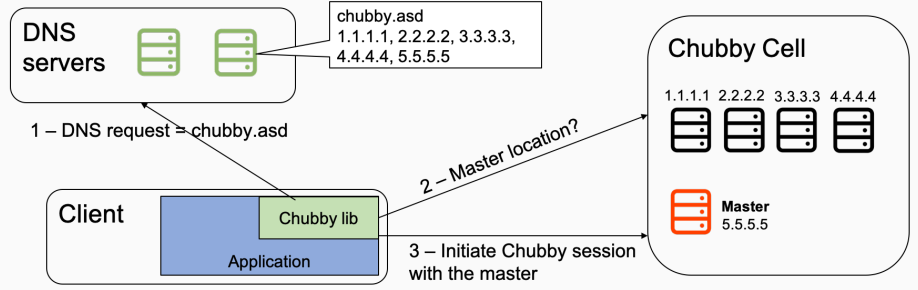
\includegraphics[width=0.6\textwidth]{images/chubby-design.png}
    \caption{\emph{Chubby} architecture}
\end{figure}

\paragraph{Chubby file system}
\emph{Chubby} exposes a file system interface simpler than that of \emph{UFS}.
The file system is a tree of files and directories with name components separated
by \texttt{/}. Each directory containes a list of files and directories which
are collectivelly called nodes. Each file containes a sequent of uninterpreted
bytes.

The interface is simpler because there are no symbolic nor hard links, no file
move, no directory times for modifications or last access, and no path-dependant
permission, meaning that permissions of a file are handled by the file itself.

\begin{figure}[h!]
    \centering
    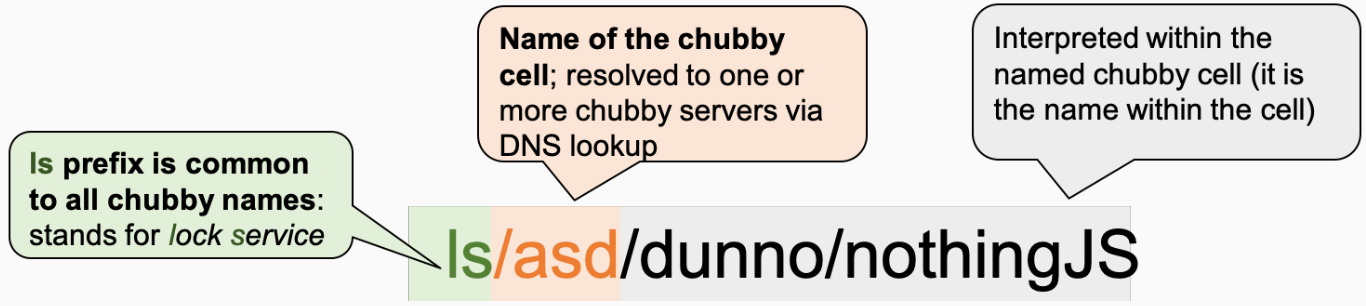
\includegraphics[width=0.6\textwidth]{images/chubby-design-fs.png}
    \caption{\emph{Chubby} file path}
\end{figure}

\noindent
Each node can be permanent (e.g. actual files and directories) or ephemeral
(e.g. temporary files) and its metadata includes three access control list
used to control read, write operations and modification of the lists themselves.
By opening a node, a client can obtain a handle, which is like a file descriptor
in Unix, and can use it to access node internal data.

\paragraph{Chubby locking system}
Each node can act as an \emph{advisory reader/writer lock}. So, if an application
wants to get access over a shared resource and operate on it, it has to acquire a
\emph{lock}. In the case of multiple clients trying to get access to the same
resource, the first one that gets the \emph{lock} becomes the one that can use it.

As previously mentioned, \emph{locks} are mapped to nodes and are of two
kinds:
\begin{itemize}
    \item \emph{Exclusive mode} (\emph{writer}): one client can hold the
    \emph{lock};
    \item \emph{Shared mode} (\emph{reader}): any number of clients can hold
    the \emph{lock};
\end{itemize}
To acquire either mode, clients must have write permission on that node.
Both modes are implemented using two other kinds of \emph{locks}:
\begin{itemize}
    \item \emph{Sequencer}: is used to ensure that the access order to a
    shared resource remains consistent. When a client acquires this \emph{lock},
    it is able to access the resource in a specific order. It also holds
    information about state of the \emph{lock};
    \item \emph{Time delay}: is used to ensure that any client attempting to
    access the resource while a \emph{lock} is in place will have to wait until
    that \emph{lock} is released;
\end{itemize}

\noindent
When using \emph{shared mode}, clients can request access to a resource in either
read or write mode. In read mode, multiple clients can access the resource
concurrently, while in write mode only one client can do it.

\paragraph{Chubby APIs: summary}
So, when using \emph{Chubby} it is possible to:
\begin{itemize}
    \item Open/close/delete nodes;
    \item Read/write full content of a node;
    \item Set access control lists;
    \item Acquire/release \emph{locks};
    \item Set/get/check sequencer;
\end{itemize}

\section{Distributed database: Google Big Table}
\emph{Google Bit Table} (\emph{GBT}) is a distributed storage system for
managing structured data. It's designed to scale, allowing it to handle petabytes
of data across thousands of servers. It is not a relational database, but a
sparse, distributed, persistent multi-dimensional sorted map (key/value store).

\begin{figure}[h!]
    \centering
    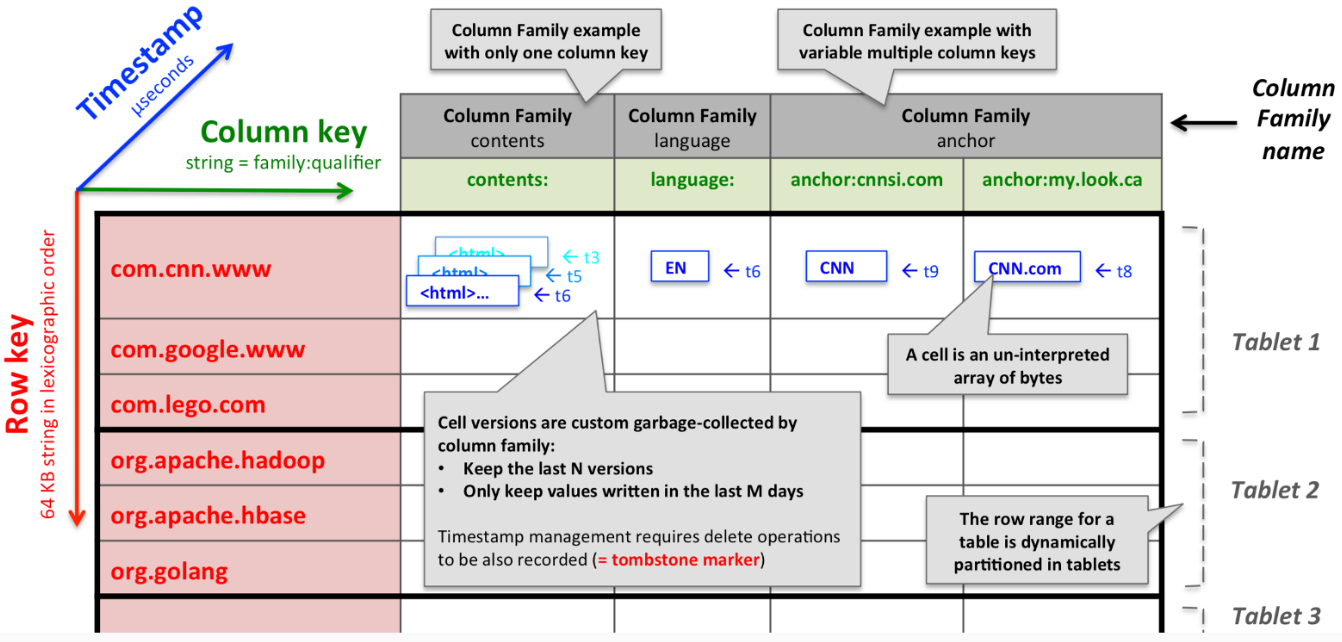
\includegraphics[width=0.8\textwidth]{images/gbt-design.png}
    \caption{\emph{GBT data model}}
\end{figure}

\subsection{How is GBT built?}

\noindent\begin{minipage}[c]{0.7\textwidth}
    \emph{GBT} uses \emph{GFS} to store data, metadata and \emph{tablet logs}.
    Data are organized in \emph{tablets} based on the \emph{SSTable} format. For
    each \emph{data tablet} there's a \emph{log tablet}, and metadata of each
    \emph{data tablet} are grouped in a collection of metadata \emph{tablets}.

    \paragraph{SSTable file format}
    \emph{SSTable} (\emph{Sorted String Table}) is a file format that stores
    data in a persistent and ordered immutable key-value map. Each \emph{SSTable}
    file contains a sequence of blocks whose size is typically 64KB.
\end{minipage}\hfill
\begin{minipage}[c]{0.28\textwidth}
    \centering
    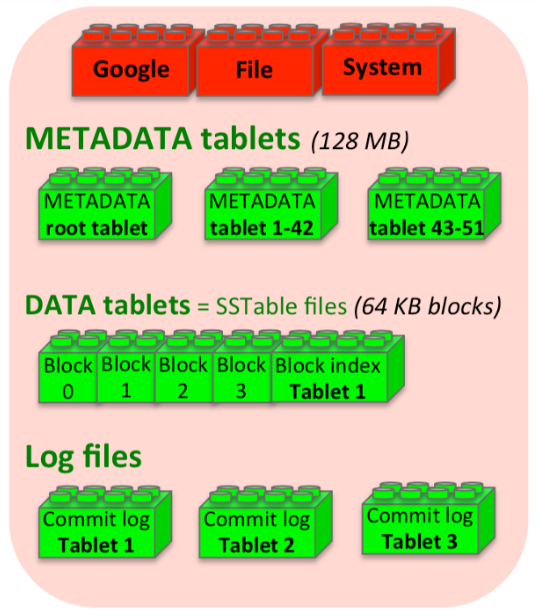
\includegraphics[width=\textwidth]{images/gbt-blocks1.png}
\end{minipage}

\noindent
Optionally, blocks can be mapped to memory, so that lookup and scan operatios
can be performed without interacting with the disk.

At the end of the file there's a block index that's used to locate other blocks.
It is loaded in memory when the \emph{SSTable} is opened and this allows to
avoid unnecessary disk interation. In fact, when looking for something,
the appropriate block can be found by performing a binary search in the in-memory
index e then loading just the correct block from the disk.

\begin{figure}[ht!]
    \centering
    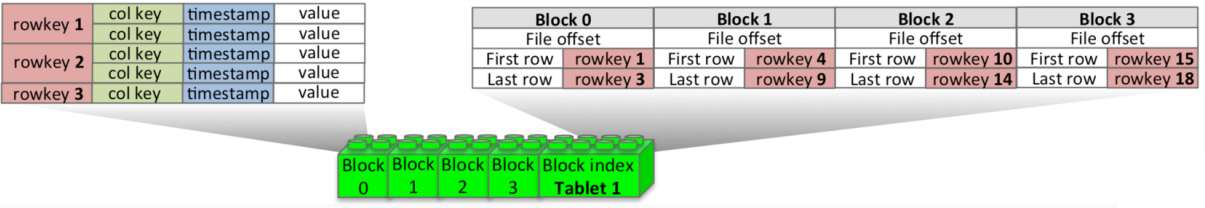
\includegraphics[width=\textwidth]{images/sstable-format.png}
    \caption{\emph{SSTable} design}
\end{figure}

\noindent\begin{minipage}[c]{0.7\textwidth}
\paragraph{Chubby as an interface for clients}
\emph{GBT} uses \emph{Chubby} as a sort of interface for client applications.
In particular, since \emph{Chubby} provides a reliable namespace that contains
directories and small files, it is used to store bootstrap location of
\emph{bigtable} data (aka \emph{root tablet}), to discover \emph{tablet servers},
and finalize their death when necessary, and to store \emph{bigtable} schema
information (i.e. column family information for each \emph{tablet}).

In addition to that, \emph{Chubby} APIs allows for access control list management,
and its design guarantees that there's at most one active \emph{master} at any
time in any \emph{cell}. Since \emph{Chubby} provides the interface to the users,
if it's unavailable, \emph{GBT} will also be unreachable.
\end{minipage}\hfill
\begin{minipage}[c]{0.28\textwidth}
    \centering
    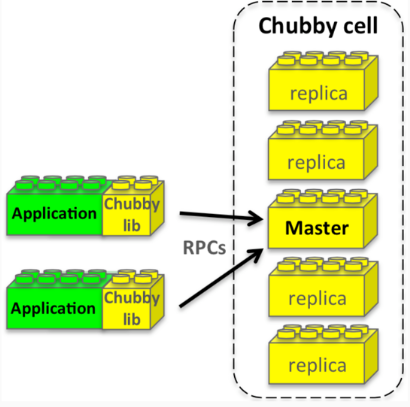
\includegraphics[width=\textwidth]{images/gbt-chubby-1.png}
\end{minipage}

\subsection{How is GBT implemented?}
\begin{figure}[h!]
    \centering
    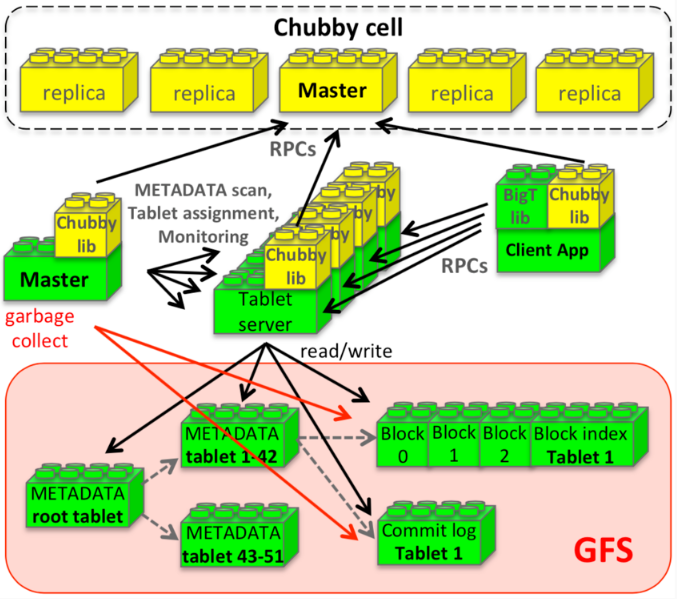
\includegraphics[width=0.6\textwidth]{images/gbt-design-detailed.png}
    \caption{\emph{GBT} architecture}
\end{figure}

\noindent
The above image shows the actual architecture of \emph{GBT}. There's one
\emph{master server} that handles:
\begin{itemize}
    \item Assigning \emph{tablets} to \emph{tablet servers};
    \item Detecting the addition and expiration of \emph{tablet servers};
    \item Balancing \emph{tablet servers} load;
    \item Garbage collection of files in \emph{GFS};
    \item Handling schema changes (\emph{tablet} creation, column family
    creation/deletion);
    \item providing metadata to the \emph{Chubby master};
\end{itemize}
Then, there are many \emph{tablet servers} and each of them is responsible for
managing a set of \emph{tablets}, handling read and write requests and even splitting
\emph{tablets} that have grown too large (usually around 100/200MB).

Finally, clients contact the \emph{Chubby master}, that responds with the
identity of the \emph{tablet server} that holds the required data, and use that
information to communicate directly with that server, bypassing the \emph{GBT
master}.

\bigskip\noindent
The API provided by \emph{GBT} is the following:
\begin{itemize}
    \item Add/remove \emph{tablet servers};
    \item Create/delete \emph{tablets};
    \item Create/delete column families;
    \item Control \emph{tablet flags} (access control rights and metadata);
    \item Control columns family flags (access control rights and metadata);
    \item Cell value: \texttt{put(rowkey, columnkey, value)},
    \texttt{get/delete(rowkey, columnkey)};
    \item Lookup value for row: \texttt{has(rowkey, columnfamily)};
    \item Lookup value from \emph{tablet}: \texttt{scan(rowfilter, columnfilter, timestampfilter)};
    \item Operations on a single row: \texttt{transactions(atomic read-modify-write sequence)};
\end{itemize}

\subsection{GBT operations}
\paragraph{Tablet location}\mbox{}

\begin{figure}[h!]
    \centering
    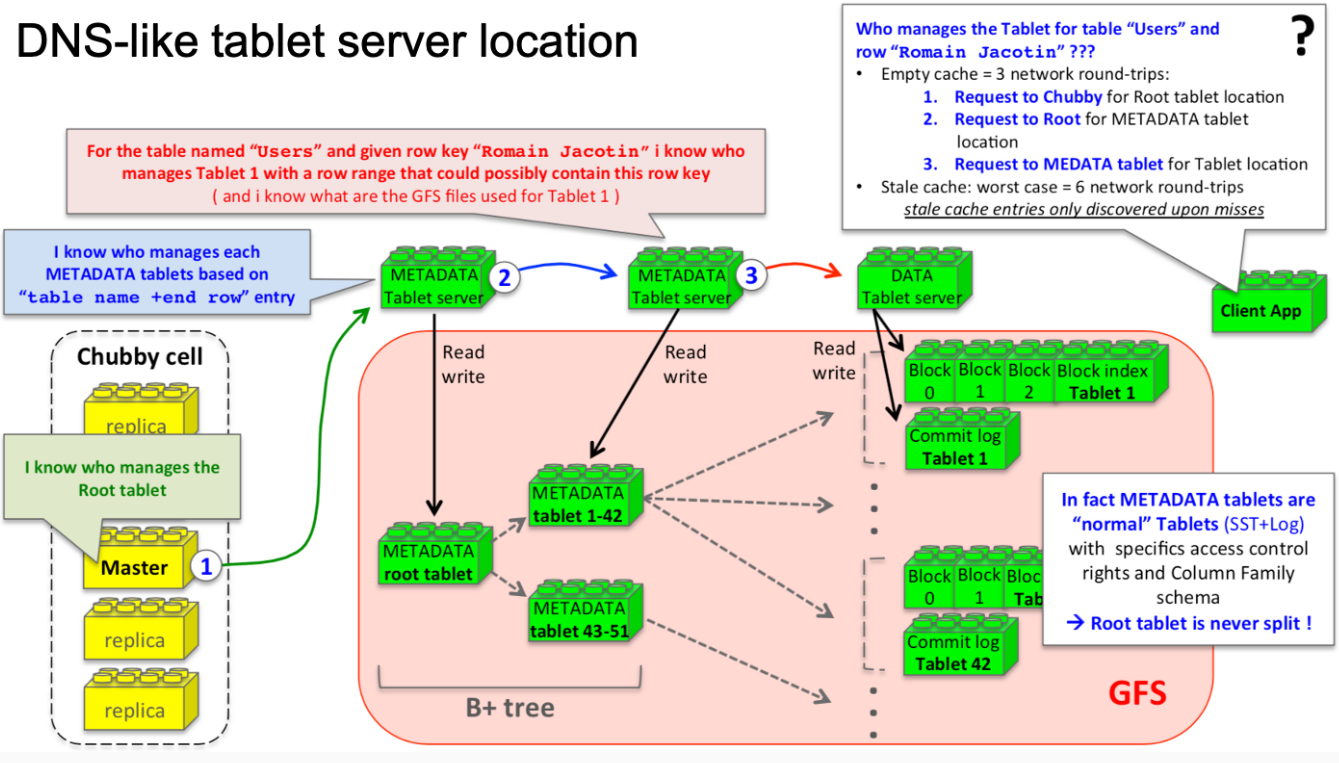
\includegraphics[width=0.7\textwidth]{images/gbt-tablet-location.png}
    \caption{\emph{Tablet} location procedure}
\end{figure}

\paragraph{Tablet assignment}
Each \emph{tablet} is assigned to one \emph{tablet server} at a time.
\emph{Master} keeps tracks of the set of live \emph{tablet servers} (via
\emph{Chubby}), current assignement of \emph{tablets} to \emph{tablet servers}
and current unassigned \emph{tablets}. When a \emph{tablet} is unassigned, the
master assigns it to an available \emph{tablet server} by sending a \emph{tablet}
load request.

\paragraph{Tablet server discovery}
When a \emph{tablet server} starts, it creates and acquires an
\emph{exclusive lock} on a uniquely-named file in a specific \emph{Chubby}
directory (\texttt{servers} directory) and the \emph{master} monitors this directory
to discover \emph{tablet servers}. A \emph{tablet server} stops serving its
\emph{tablets} if it loses its \emph{exclusive Chubby lock}, and if the
\emph{Chubby} file no longer exists, then the \emph{tablet server} will never
be able to serve again, so it kills itself.

\paragraph{Tablet server monitoring}
The \emph{master} is responsible for detecting when a \emph{tablet server} is no
longer serving its \emph{tablets}, and for reassigning those \emph{tablets},
and it does so by periodically asking each \emph{tablet server} for the status of
its \emph{lock}. If a \emph{tablet server} reports that it has lost its
\emph{lock}, or if the \emph{master} was unable to reach a server during its last
attempt, the \emph{master} attempts to acquire the \emph{lock} for the
\emph{Chubby} file.

If it succedes, then \emph{Chubby} is live and the \emph{tablet server} is dead
or isolated, so the \emph{master} deletes its server file to ensure that the
\emph{tablet server} can never serve again. Then, the \emph{master} can put
all the \emph{tablets} that were previously assigned to that \emph{tablet
server} into the set of unassigned \emph{tablets}.

\paragraph{Master startup}
When a \emph{master} is started by the cluster management system, it needs to
discover the current \emph{tablet} assignments before it can change them. This
is a five-steps procedure:
\begin{enumerate}
    \item The \emph{master} grabs a \emph{unique master lock} in \emph{Chubby}
    to prevent concurrent \emph{master} instantiations;
    \item It scans the \texttt{servers} directory in \emph{Chubby} to find all
    live
    \emph{tablet servers};
    \item It communicates with every live \emph{tablet server} to discover what
    \emph{tablets} are already assigned to each server;
    \item It adds the \emph{root tablet} to the set of \emph{unassigned tablets},
    if an assignment for it wasn't previuosly discovered;
    \item Finally, the \emph{master} scans the \emph{METADATA tablet} to learn
    the complete set of \emph{tablets} and eventually detect unassigned ones;
\end{enumerate}

\paragraph{Master isolated}
To ensure that a \emph{bigtable} cluster is not vulnerable to networking issues
between the \emph{master} and \emph{Chubby}, the \emph{master} kills itself if
its \emph{Chubby} session expires (\emph{master} failures do not change the
assignment of \emph{tablets} to \emph{tablet servers}).

\paragraph{Tablet merging/splitting}
The set of existing \emph{tablets} only changes when a \emph{tablet} is created
or deleted. Two existing \emph{tablets} can be merged to form a larger one, and
a large one can be split in two smaller \emph{tablets}. \emph{Tablets} merging
must be initiated by the \emph{master} while \emph{tablet} splitting can be
initiated by \emph{tablet servers}. In this case, the \emph{tablet server} that
manages the \emph{tablet} to split, commits the split by recording information
for the new \emph{tablet} in the \emph{METADATA tablet}. After that, the server
notifies the \emph{master}.

\paragraph{Tablet serving}\mbox{}

\bigskip\noindent\begin{minipage}[c]{0.65\textwidth}
    Steps for a write operation:
    \begin{enumerate}
        \item \emph{Tablet server} checks if the request is well-formed;
        \item \emph{Tablet server} checks if sender is authorized to write by
        looking up the list of permitted writers in a \emph{Chubby} file;
        \item The valid mutation is written to commit log that stores redo
        records (commits can be grouped to increase throughtput);
        \item After mutation is committed, its content is inserted into
        memtable (i.e. in a memory sorted buffer);
    \end{enumerate}
\end{minipage}\hfill
\begin{minipage}[c]{0.33\textwidth}
    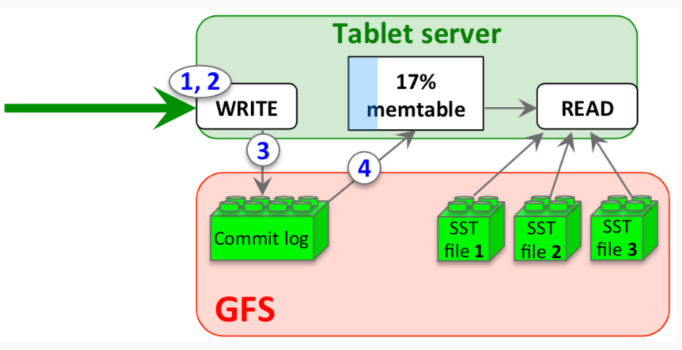
\includegraphics[width=\textwidth]{images/gbt-tablet-write.png}
\end{minipage}

\bigskip\noindent\begin{minipage}[c]{0.65\textwidth}
    Steps for a read operation:
    \begin{enumerate}
        \item \emph{Tablet server} checks if the request is well-formed;
        \item \emph{Tablet server} checks if sender is authorized to read by
        looking up the list of permitted readers in a \emph{Chubby} file;
        \item The valid read operation is executed on a merged view of the
        sequence of \emph{SSTables} and the memtable;
    \end{enumerate}
\end{minipage}\hfill
\begin{minipage}[c]{0.33\textwidth}
    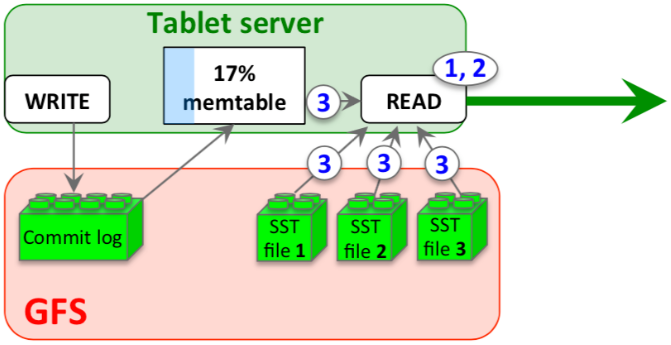
\includegraphics[width=\textwidth]{images/gbt-tablet-read.png}
\end{minipage}

\bigskip\noindent\begin{minipage}[c]{0.65\textwidth}
    Steps for a \emph{tablet} recovery operation:
    \begin{enumerate}
        \item \emph{Tablet server} reads its metadata from the \emph{METADATA
        table} (lists of \emph{SSTables} that comprise a \emph{tablet} and        a set of a redo points, which are
        pointers into any commit logs that may contain data for the \emph{tablet});
        \item \emph{Tablet server} reads the indices of the \emph{SSTables}
        into memory and reconstructs the memtable by applying all the updates
        that have been committed since the redo points;
    \end{enumerate}
\end{minipage}\hfill
\begin{minipage}[c]{0.33\textwidth}
    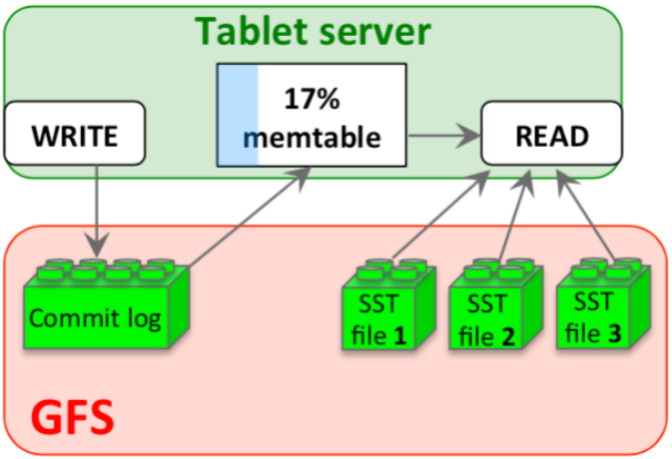
\includegraphics[width=\textwidth]{images/gbt-tablet-recovery.png}
\end{minipage}

\paragraph{Tablet minor compaction}
When memtable size reaches a threshold, the memtable is frozen, a new memtable
is created, and the frozen memtable is converted to a new \emph{SSTable} and
written to \emph{GFS}. The goals of this operation are two: shrink the memory
usage of the \emph{tablet server} and reduce the amount of data that has to be
read from the commit log during a recovery.

\begin{figure}[h!]
    \centering
    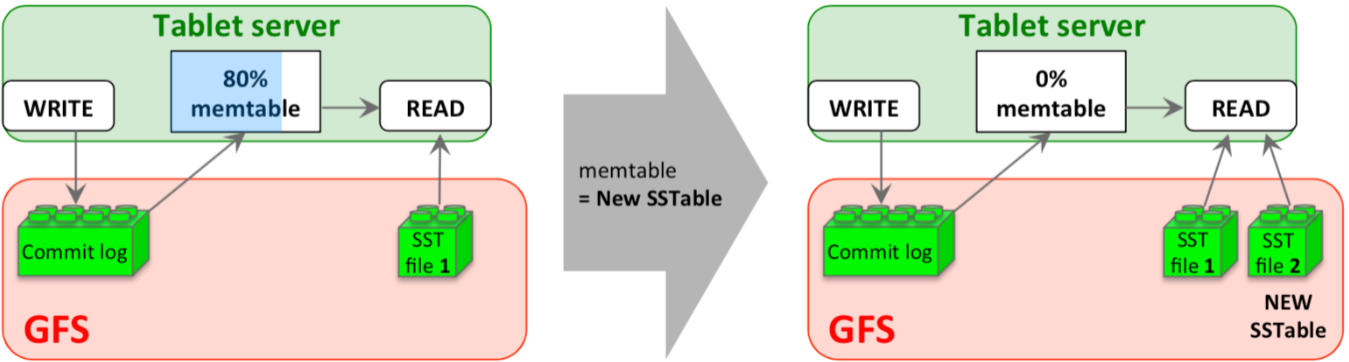
\includegraphics[width=0.8\textwidth]{images/gbt-tablet-minor-comp.png}
    \caption{\emph{Tablet minor compaction}}
\end{figure}

\paragraph{Tablet merging compaction}
The problem of \emph{tablet minor compaction} is that every \emph{minor
compaction} creates a new \emph{SSTable} and in the long run there might be
an inconveniently large amount of \emph{SSTables}. The solution to this is
doing a periodic merging of a few \emph{SSTables} and the memtable.

\begin{figure}[ht!]
    \centering
    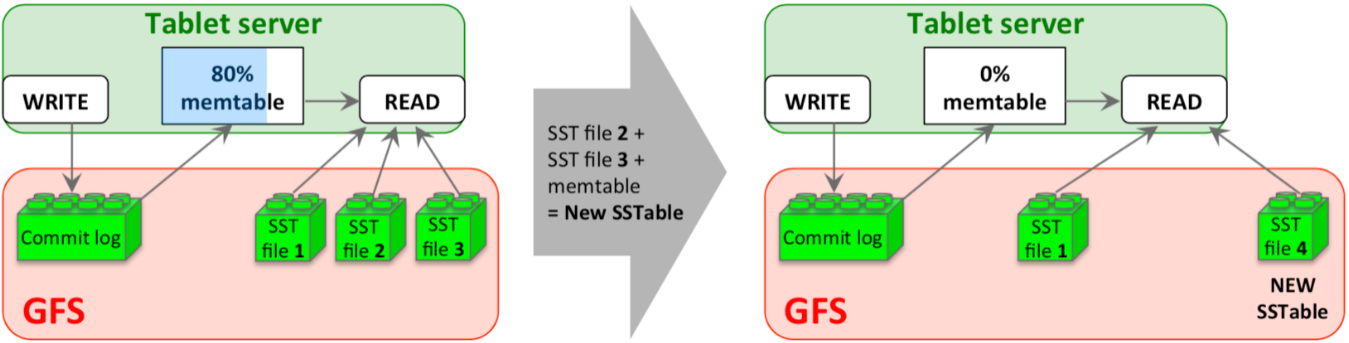
\includegraphics[width=0.8\textwidth]{images/gbt-tablet-merge-comp.png}
    \caption{\emph{Tablet merging compaction}}
\end{figure}

\paragraph{Tablet major compactor}
It is a \emph{merging compaction} that rewrites all \emph{SSTables} into
exactly one \emph{SSTable} that contains no deletion information or deleted
data. \emph{Bigtable} cycles throught all of its \emph{tablets} and regularly
applies \emph{major compaction} to them, that is to say, that it reclaims
resources used by deleted data in a timely fashion.

\begin{figure}[h!]
    \centering
    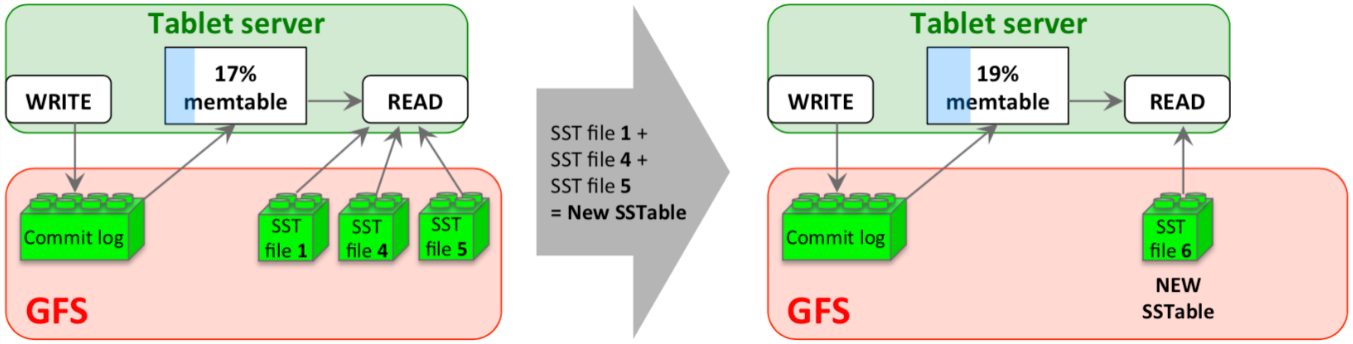
\includegraphics[width=0.8\textwidth]{images/gbt-tablet-major-comp.png}
    \caption{\emph{Tablet major compaction}}
\end{figure}

\section{Distributed object storage: OpenStack Swift}
\emph{OpenStack Swift} (\emph{OSS}) is a distributed object storage system
designed to scale from a single machine to thousands of servers. It's optimized
for \emph{multi-tenancy} and high concurrency. It's ideal for backups, web and
mobile content, and any other unstructured data that can grow without bound.
Among the features of \emph{OSS} there are consistency, because every access to
an item will return its most recent value, high availability, possibility to
rely on commodity hardware, authentication procedures and possibility the
possibility to set up quotas, access control lists and various storage policies.

Since this is not a distributed file system, it's impossible to mount it, create
a file hierarchy, create a file system from a certain state of the service, and
even store objects which exedes a certain size (but this might not always be the
case).

\paragraph{OSS hierarchycal structure}
Despite not allowing file hierarchies, \emph{OSS} is itself organized in a
hierarchical way. Specifically, it is made up of three levels:
\begin{enumerate}
    \item \emph{Account}: is the top level and is associated to every service
    user. It defines a namespace in which the owner can create and manage its
    own \emph{containers};
    \item \emph{Container}: is a namespace for \emph{objects} and can be thought
    as a folder. Access control list, along with storage policies can be
    associated to each \emph{container};
    \item \emph{Object}: represent the actual data and is handled as an
    uncompressed and unencrypted format with metadata;
\end{enumerate}

\begin{figure}[h!]
    \centering
    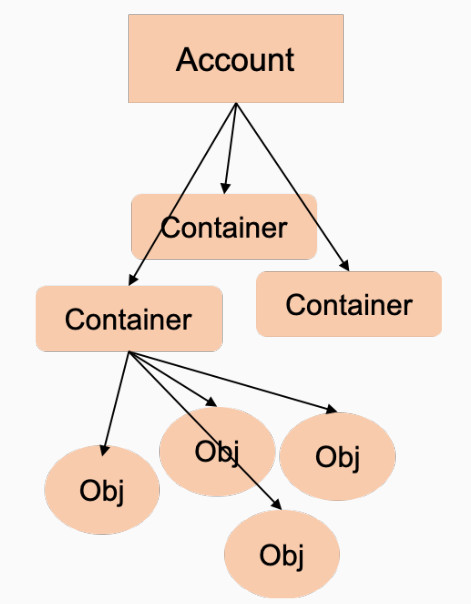
\includegraphics[width=0.4\textwidth]{images/oss-hierarchy.png}
    \caption{\emph{OSS} hierarchy}
\end{figure}

\subsection{OSS architecture}
\begin{figure}[h!]
    \centering
    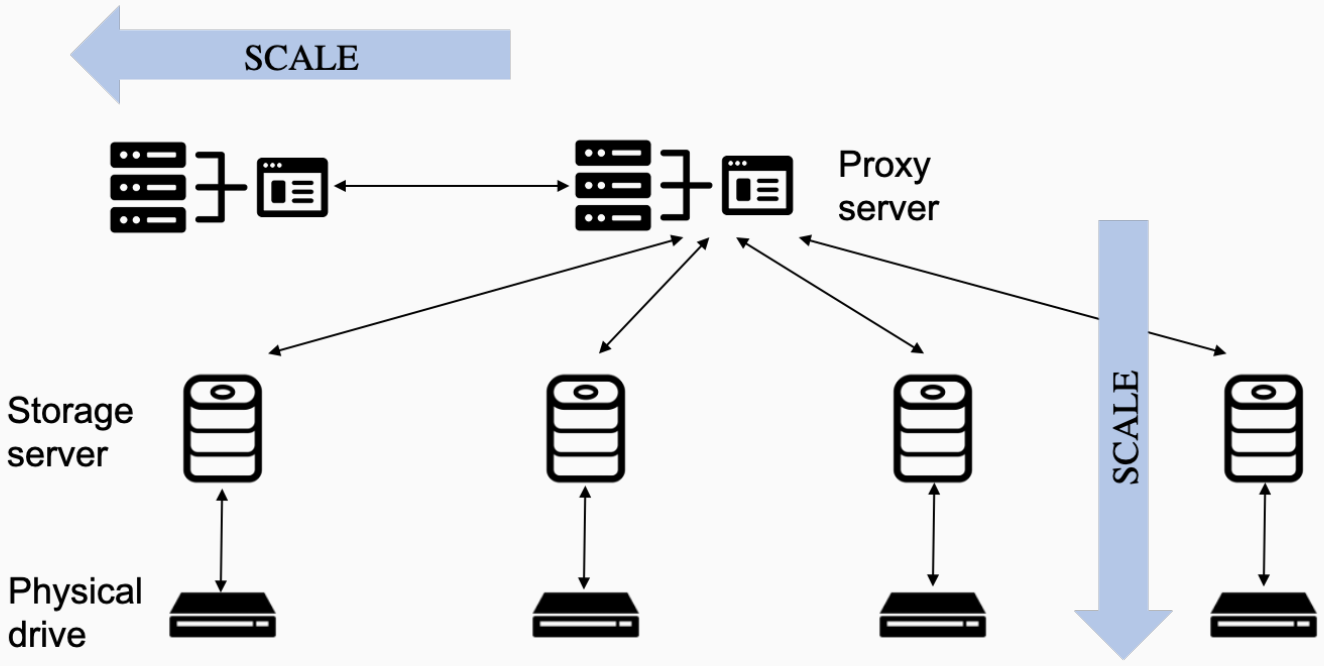
\includegraphics[width=0.8\textwidth]{images/oss-architecture.png}
    \caption{\emph{OSS} architecture}
\end{figure}

\noindent
The \emph{proxy server} is responible for keeping together the architecture.
For each request it receives, it looks up the location of the \emph{account},
\emph{container} or \emph{objet} in the \emph{ring}, and routes the request
accordingly. More precisely, the \emph{proxy server} serves as the interface
to the users. It's responsible to implement the \emph{OSS} APIs, accept and
answer to user requests, handle failures and make sure that the communication
with \emph{storage servers} is up and working.

Then, there are two more categories of server:
\begin{itemize}
    \item \emph{Storage servers}:
    \begin{itemize}
        \item \emph{Object servers}: servers that store, retrive and delete
        \emph{objects} stored in their local devices;
        \item \emph{Container servers}: servers that handle listings of
        \emph{objects}. They don't know where the \emph{objects} are, but to
        what \emph{container} they belong. Each server keeps the listing in a
        replicated SQLite database together with statistics about the
        \emph{containers} it controls;
        \item \emph{Account servers}: they're the same as \emph{container servers},
        but keep listings of \emph{containers} instead of \emph{objects};
    \end{itemize}
    \item \emph{Consistency servers}:
    \begin{itemize}
        \item \emph{Replicator}: keeps the system in a consistent state in case
        of temporary error conditions (e.g. drive failures or netwok outages);
        \item \emph{Updater}: when \emph{containers} or \emph{accounts} data
        cannot be immediately updated, in the case of conjestion or failures,
        the updates are queued locally on the file system and carried out by
        the \emph{updater} when possible;
        \item \emph{Auditors}: scans local servers checking for integrity of
        \emph{objects}, \emph{containers} and \emph{accounts}. All the errors
        are logged and if a corrupted file is found, that file is quarantined
        and will be replaced by the \emph{replicator} with a correct replica;
    \end{itemize}
\end{itemize}

\paragraph{OSS API}
Here's a list of some funtions exposed by \emph{OSS} APIs:
\begin{itemize}
    \item \texttt{GET}: download \emph{objects}, list content of \emph{containers} or
    \emph{accounts};
    \item \texttt{PUT}: uploads \emph{objects}, creates \emph{containers},
    overwrites metadata headers;
    \item \texttt{POST}: creates \emph{containers} if they do not exist, updates
    metadata (\emph{accounts} or \emph{containers}) and overwrites metadata
    (\emph{objects});
    \item \texttt{DELETE}: deletes empty \emph{objects} and empty \emph{containers};
    \item \texttt{HEAD}: retrieves header information for \emph{accounts}, \emph{containers}
    or \emph{objects};
\end{itemize}

\begin{note}
    \emph{OSS} provides a REST API.
\end{note}

\paragraph{OSS rings}
A \emph{ring} is a data structure in which each node is connected to its
neighbours forming a loop. Each node in the \emph{ring} is a \emph{storage server}.
\emph{Rings} are managed by a \emph{ring component} and is used to determine
where data should be stored and even redistribute data evenly aroung nodes,
according to weights based on the available capacity of each node.

A \emph{ring} keeps a mapping of the nodes using availability zones, partitions
and replicas. Each partition is replicated across the cluster (group of
\emph{storage servers} interconnected in a \emph{ring}) according to the
storage policies (by default 3 replicas per partition). The location of each
partition is also stored in the mapping maintained by the \emph{ring}. In fact,
each node in the \emph{ring} is assigned a certain number of partions, and each
partition is responsible for storing a certain amount of data.

Replicas inside each partition are isolated in as many distinct regions, zones,
servers and devices as possible, so as to reduce failure domains. Regions are
based on their geographical location (e.g. West Europe), while zones are more
abstract (e.g. city, power separtion, network separation, or any other attribute
that would lessen multiple replicas being available at the same time). There
might be less failure domains than replicas of a partition.

\begin{eg}[Steps for a PUT request]
    Let's see the steps needed for a simple \texttt{PUT} request.

    \begin{figure}[h!]
        \centering
        \subfloat[Client sends the request]{
            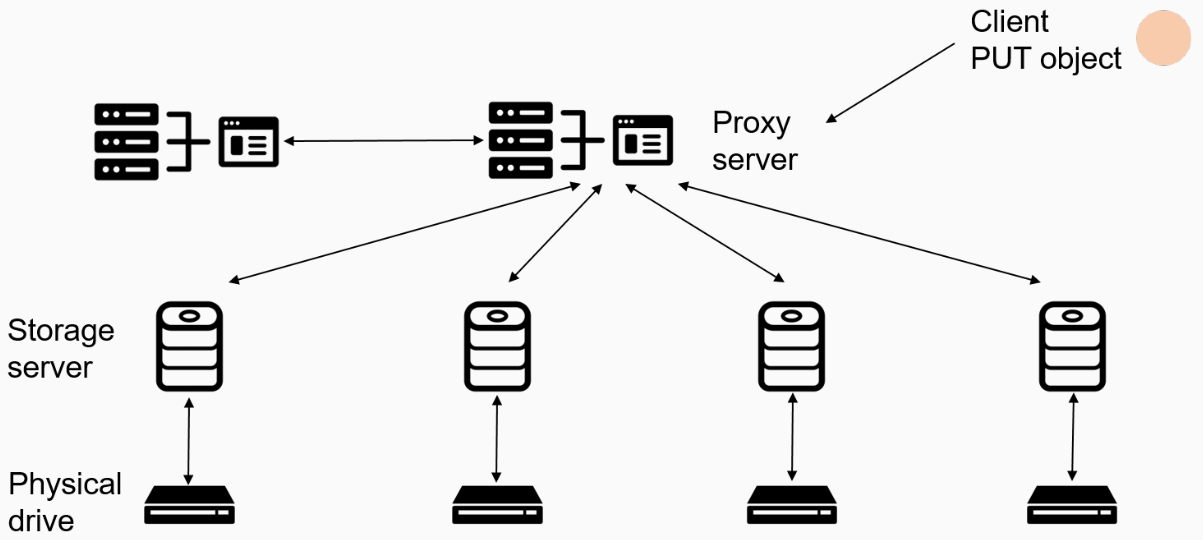
\includegraphics[width=0.48\textwidth]{images/oss-put-1.png}
        }\hfill
        \subfloat[\emph{Proxy} receives the request\\and begins processing it]{
            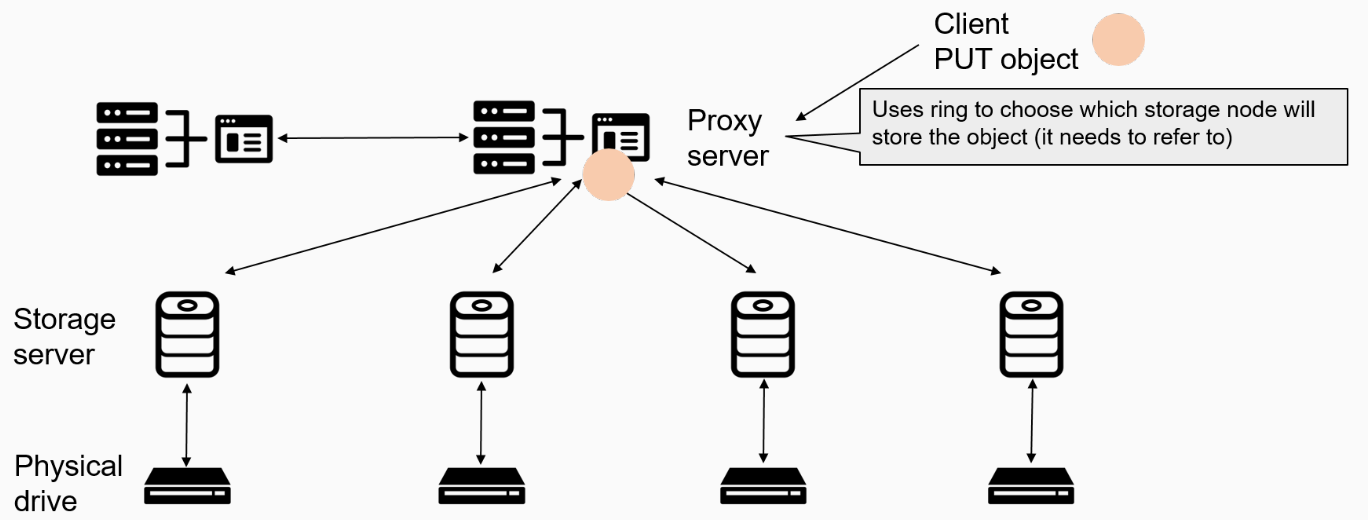
\includegraphics[width=0.48\textwidth]{images/oss-put-2.png}
        }\\
        \subfloat[A \emph{storage server} is chosen\\as responsible for storing]{
            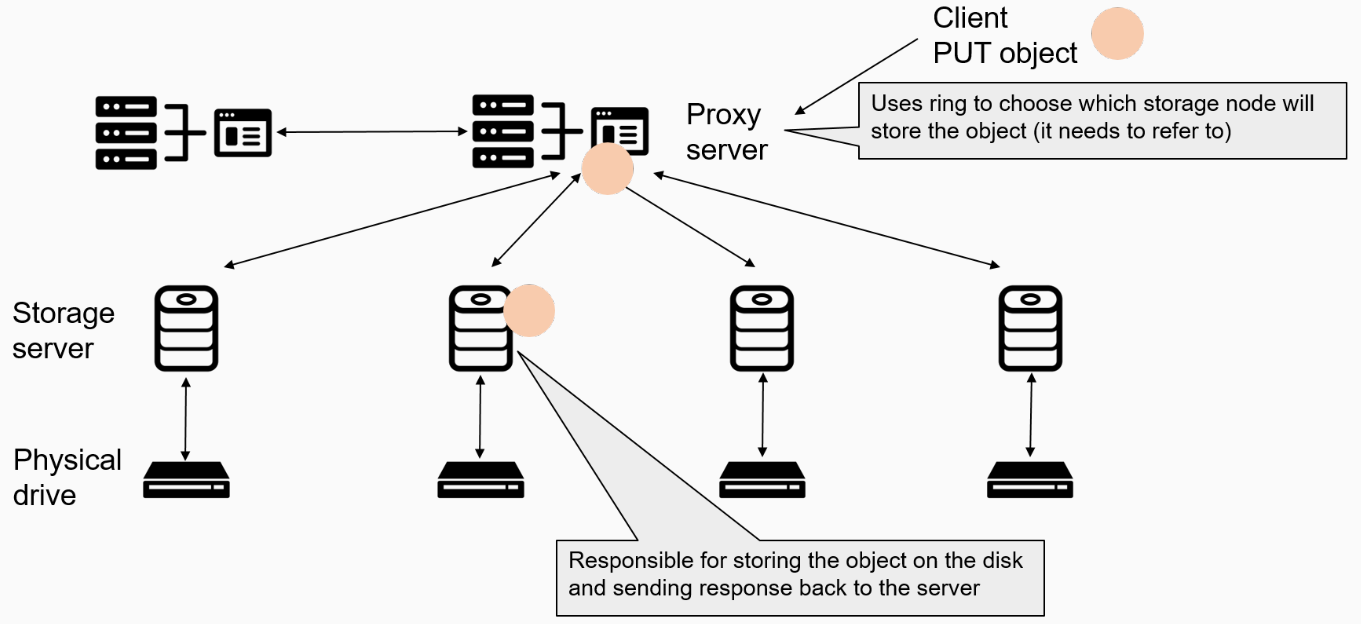
\includegraphics[width=0.48\textwidth]{images/oss-put-3.png}
        }\hfill
        \subfloat[The server and its neighbours\\store data]{
            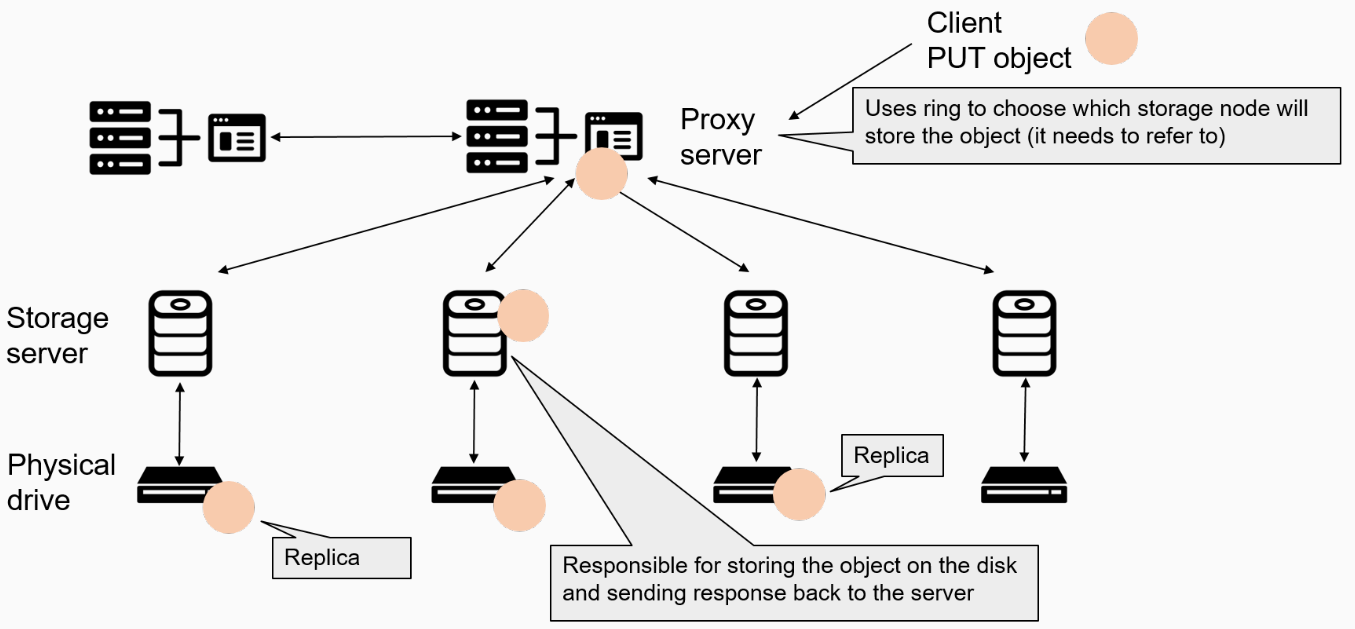
\includegraphics[width=0.48\textwidth]{images/oss-put-4.png}
        }\\
        \subfloat[The \emph{proxy} responds to the client]{
            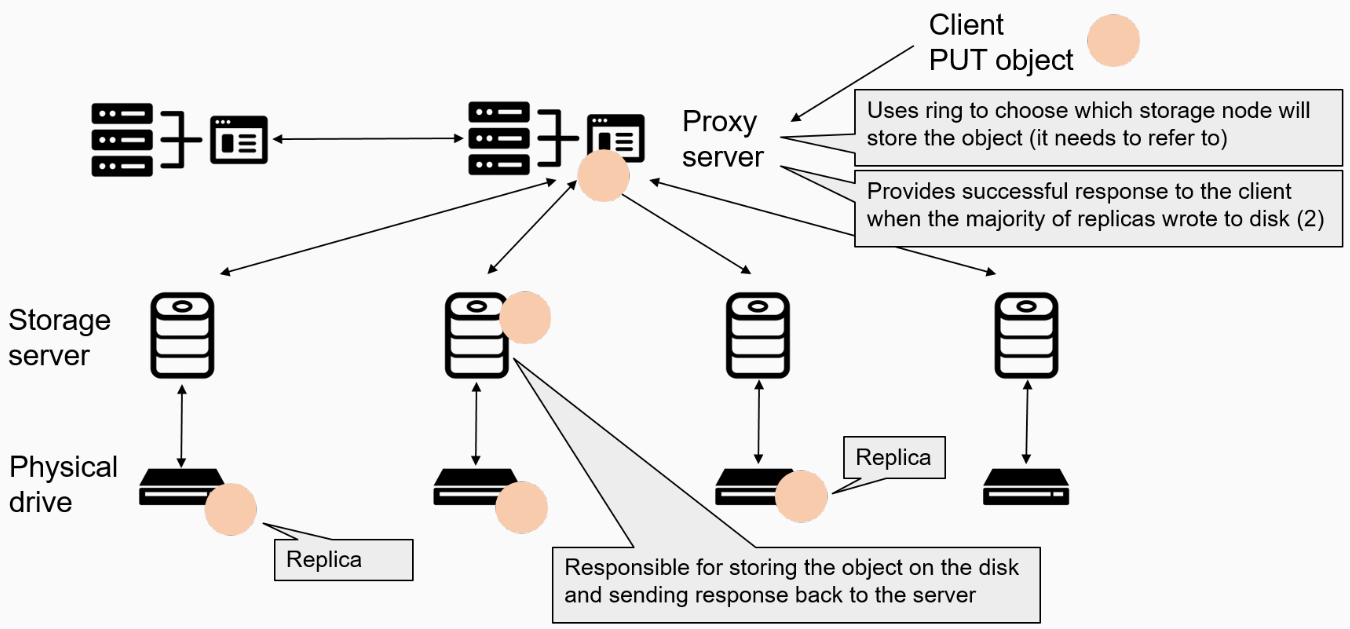
\includegraphics[width=0.48\textwidth]{images/oss-put-5.png}
        }
    \end{figure}

    \noindent
    If the \emph{storage server} that's handling the data has a failed drive,
    data are passed to another server. For example, it might be passed to the
    fourth server in the image:

    \begin{figure}[h!]
        \centering
        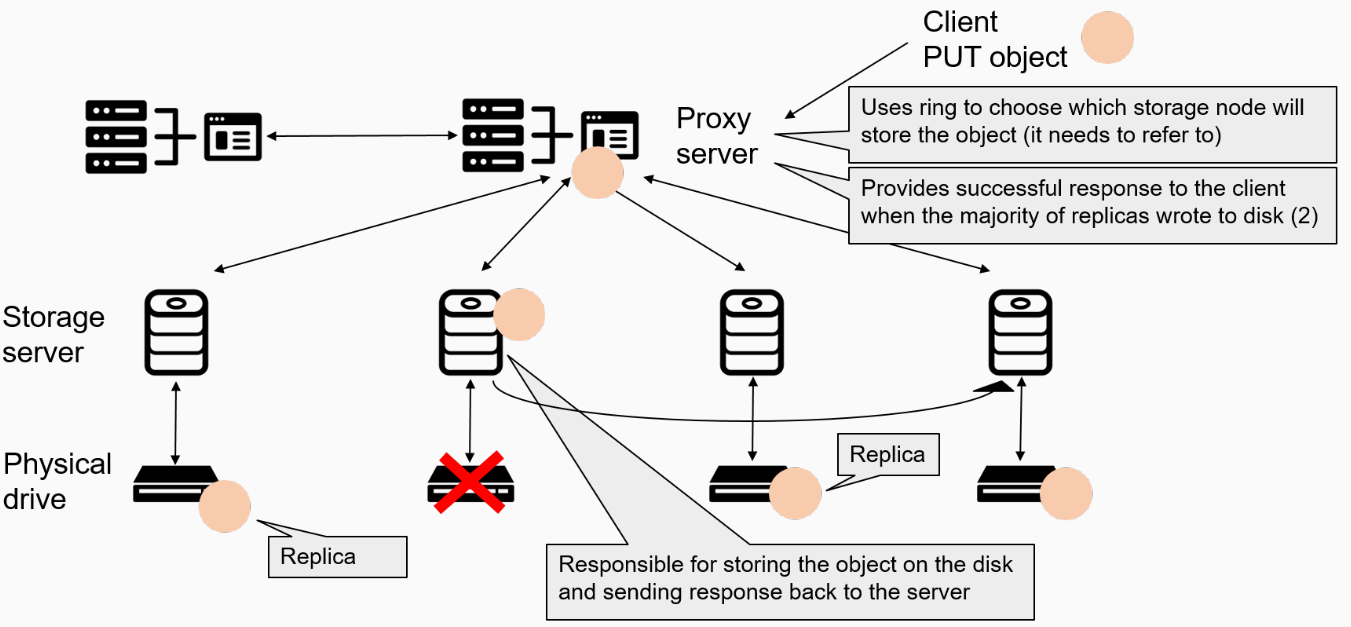
\includegraphics[width=0.48\textwidth]{images/oss-put-6.png}
    \end{figure}
\end{eg}